% WACV 2027 paper — "From Revit to Robot"
% Built on the CVF author kit (cvpr.sty); banner set to WACV via \confName.
% Toggle anonymity: use \usepackage[review]{cvpr} for the anonymous review build,
% or \usepackage{cvpr} (current) for a named, camera-ready-style draft.

\documentclass[10pt,twocolumn,letterpaper]{article}

\usepackage{cvpr}                 % named/final-style draft
% \usepackage[review]{cvpr}       % anonymous review build (line numbers, paper ID)

\usepackage{graphicx}
\usepackage{amsmath}
\usepackage{amssymb}
\usepackage{booktabs}
\usepackage{array}
\usepackage{textcomp}
\usepackage{xcolor}
\usepackage{multirow}

\definecolor{cvprblue}{rgb}{0.21,0.49,0.74}
\usepackage[pagebackref,breaklinks,colorlinks,allcolors=cvprblue]{hyperref}
\usepackage[capitalize]{cleveref}   % \cref / \Cref (load after hyperref)
\crefname{table}{Tab.}{Tabs.}
\crefname{figure}{Fig.}{Figs.}
\crefname{section}{Sec.}{Secs.}

\def\paperID{*****}
\def\confName{WACV}
\def\confYear{2027}

% Placeholder box for figures not yet inserted.
\newcommand{\figbox}[2]{%
  \fbox{\parbox[c][#1][c]{0.96\linewidth}{\centering\itshape\small #2}}}

\title{From Revit to Robot: BIM-Derived Digital Twins for\\
Sim-to-Real Autonomous Building Patrol}

\author{%
Adrian Manchado\thanks{Corresponding author.} \quad Tanner Cellio \quad Owen Pacetti \quad Steven Thomas\\
Joseph Loduca \quad Nicolas Picha \quad Diego Gonzalo \quad Delsoro Some\\
College of Dwight and Dian Diercks School of Advanced Computing\\
Milwaukee School of Engineering, 1025 N Broadway St, Milwaukee, WI 53202\\
{\tt\small \{manchadoa, celliot, pacettio, thomasst, loducaj, pichan, gonzaloborged, somed\}@msoe.edu}
}

\begin{document}
\maketitle

\begin{abstract}
Autonomous indoor service robots are normally trained only after a building is
finished and accessible, which is slow, costly, and risky on a live campus. We
present \textbf{Revit to Robot}, an end-to-end pipeline that turns a building's
architectural design data into a physics-accurate training ground for an
autonomous mobile robot \emph{before the physical structure is complete}.
Starting from Revit/BIM models of the MSOE campus, we automatically convert
architecture into simulation-ready USD digital twins in NVIDIA Isaac Sim,
applying triangle-mesh colliders to static structure (walls, floors, glazing,
stairs) and articulated revolute joints with calibrated hinge offsets and motor
torque to make every hinged door functional. From each twin we extract a 2D
occupancy map by ray-tracing the model from 75--175 vantage points per floor
($102.6\,\text{m}\times100.3\,\text{m}$, ${\sim}99\%$ floor coverage), place a
navigation graph with NVIDIA SWAGGER, and compute an efficient door-inspection patrol route
via Dijkstra distance tables refined with greedy nearest-neighbor and 2-opt
search (a traveling-salesman formulation). A differential-drive Nova Carter robot
(``ROSCOE'') drives this route with the ROS\,2 Nav2 stack, using its onboard
$360^\circ$ LiDAR for real-time local planning and obstacle avoidance between
waypoints. For environmental awareness, we fine-tune a Qwen3-VL-2B
vision-language model with LoRA ($\approx1.6\%$ of parameters trained) to detect
the two highest-priority anomalies identified by campus public safety ---
open/unsecured doors and cracked glass --- using only synthetic imagery generated
by programmatically manipulating the digital twin's internal state, which yields
free ground-truth labels across thousands of randomized lighting, material, and
viewpoint conditions. The fine-tuned model reaches $97.4\%$ / $97.2\%$ accuracy
on held-out door / glass frames, retains $90.2\%$ on a held-out-instance door
test, and transfers to real-world imagery of an already-built campus building at
$93.0\%$ accuracy. The entire system is repeatable for any building with BIM
data; we apply it to a six-building digital campus, consuming over 3{,}500 GPU
jobs and 2{,}000 GPU-hours on MSOE's Rosie supercomputer. Our results show that
BIM data --- typically treated as static documentation --- can serve as a
scalable, automatically labeled training substrate for sim-to-real robot
autonomy.
\end{abstract}

\section{Introduction}

Simulation-based training has become the dominant approach for developing robot
navigation systems. It offers safe, scalable, and repeatable experimentation
without the cost or risk of real-world trials. However, most robots are trained
in generic virtual scenes that do not match the specific geometry of their actual
deployment sites. Building these high-fidelity environments by hand is slow,
expensive, and requires specialized expertise. This bottleneck limits
simulation-based robot training to well-resourced teams and constrains most
deployed systems to generic environments that do not reflect where they will
actually operate.

Building Information Modeling (BIM) offers a path forward that has gone largely
unexploited in the robotics community. BIM tools such as Autodesk Revit are
already used by architects and facility managers to produce precise, semantically
rich 3D models of buildings as part of standard construction and maintenance
workflows. These models contain exactly the geometric and spatial information
needed to construct a simulation environment, yet this data is rarely connected
to robot training.

This paper presents a framework to bridge that gap. Our pipeline converts Revit
files into physics-accurate digital twins in NVIDIA Isaac Sim without manual
scene authoring. From each twin we (i) extract a 2D occupancy map and a
navigation graph for deterministic patrol-route planning, (ii) drive a
differential-drive robot along those routes with the ROS\,2 Nav2 stack for
real-time, LiDAR-based obstacle avoidance, and (iii) fine-tune a vision-language
model (VLM) for anomaly detection using only synthetic imagery whose ground-truth
labels come for free from the twin's internal physics and material state.

We demonstrate the framework on autonomous security patrol --- a domain where the
need for site-specific training is acute and the connection to real facility data
is natural. The system is developed in coordination with MSOE's Public Safety
Office and is anchored to the Robert D. Kern Engineering Innovation Center, a
four-story facility currently under construction. Because the building does not
yet physically exist, it cannot be entered, photographed, or used for data
collection --- making a BIM-derived digital twin not merely convenient but the
only way to train for it ahead of opening.

An earlier version of this system trained a reinforcement-learning (RL) policy in
Isaac Lab for local navigation. We found that a classical, well-engineered
navigation stack (ROS\,2 Nav2) reached reliable obstacle avoidance and route
following far faster, with no reward engineering and a smaller sim-to-real gap for
locomotion, so Nav2 is the navigation method used throughout this paper; the RL
effort is retained only as an archived exploration.

The contributions of this paper are:
\begin{enumerate}
\itemsep0.1em
\item \textbf{An end-to-end pipeline from architectural BIM data to a
simulation-ready digital twin} in NVIDIA Isaac Sim, requiring no manual scene
authoring, and scaled to a six-building digital campus.
\item \textbf{An automatic navigation-graph and patrol-route pipeline} that
derives a 2D occupancy map by ray-tracing the twin, places a navigation graph
with NVIDIA SWAGGER, and computes efficient door-inspection routes as a
traveling-salesman problem (Dijkstra distance tables + greedy nearest-neighbor +
2-opt).
\item \textbf{A deployment of the ROS\,2 Nav2 stack inside the BIM-derived twin}
that drives a Nova Carter robot through planned routes using onboard LiDAR for
local planning and obstacle avoidance, with documented parameter choices that
make off-the-shelf Nav2 work in long architectural corridors.
\item \textbf{A label-free VLM fine-tuning methodology for sim-to-real anomaly
detection} that adapts a Qwen3-VL-2B model with LoRA and vision-projector
co-training to detect two public-safety anomalies --- open/unsecured doors and
cracked glass --- from synthetic renders alone, and that transfers to real-world
building imagery at over $90\%$ accuracy.
\end{enumerate}

\begin{figure}[t]
  \centering
  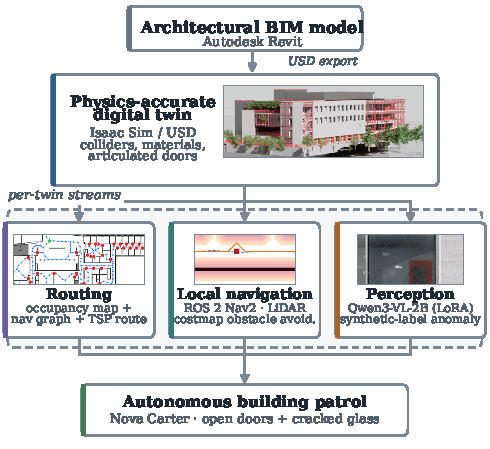
\includegraphics[width=0.86\linewidth]{figures/fig_overview.pdf}
  \caption{Overview of the integrated BIM-to-Robot pipeline. A single Autodesk
  Revit model becomes a physics-accurate Isaac Sim digital twin that feeds three
  streams --- navigation-graph routing, ROS\,2 Nav2 local navigation, and
  Qwen3-VL anomaly perception --- converging on an autonomous Nova Carter patrol.}
  \label{fig:overview}
\end{figure}

\section{Related Work}

\noindent\textbf{Simulation-based navigation and Isaac Sim.}
Simulation-based training is a cornerstone of mobile-robot development because it
enables policy learning in safe, repeatable environments before physical
deployment, with extensive work on obstacle avoidance and goal-directed indoor
navigation~\cite{sun2021motion}. NVIDIA Isaac Sim has become a leading platform
for high-fidelity robot simulation, with Isaac Lab extending it for massively
parallel learning~\cite{mittal2025isaaclab}, and Salimpour \etal~\cite{salimpour2025sim2real}
demonstrated end-to-end sim-to-real transfer of navigation policies on physical
ROS\,2 robots using this stack. A limitation shared by these and most
simulation-based approaches is that the training environments are generic,
hand-authored scenes with no relationship to the actual deployment site. Our
framework replaces the hand-authored environment with one automatically derived
from the target building's own architectural data.

\noindent\textbf{Classical navigation (Nav2).}
Rather than learn a local-navigation policy from scratch, we drive the robot with
the ROS\,2 Nav2 stack~\cite{macenski2020marathon2}, the de facto standard for
autonomous ground-robot navigation. Nav2 composes a global planner, a local
trajectory controller, probabilistic localization (AMCL), and a behavior tree for
recovery, over layered costmaps fused from LiDAR. Its components are mature and
well-studied, which lets us focus the research contribution on the BIM-to-twin and
perception pipelines rather than on re-deriving local navigation.

\noindent\textbf{BIM for robot navigation.}
BIM has been explored as a source of spatial knowledge for robot navigation, with
prior work showing that BIM/IFC data can generate navigation maps, occupancy
grids, and waypoint sequences for autonomous
inspection~\cite{palacz2019indoor,labbe2021semantic,gopee2023ifc,chen2024reality}.
A fundamental limitation shared across these works is the extraction of
simplified 2D or graph-based representations rather than preserving full 3D
geometry, which precludes high-fidelity physics simulation or in-twin policy
training. Our framework converts BIM geometry to the Universal Scene Description
(USD) format and loads the complete 3D scene into Isaac Sim, enabling
physics-accurate simulation, articulated doors, and onboard sensor rendering
inside the as-designed building.

\noindent\textbf{Vision-language models and parameter-efficient fine-tuning.}
VLMs enable semantic scene understanding without task-specific classifiers, but
models pretrained on real imagery suffer a sim-to-real gap when applied to
synthetic renders. Parameter-efficient methods, particularly Low-Rank Adaptation
(LoRA)~\cite{hu2021lora}, adapt large models to new visual domains while
preserving general reasoning. We apply LoRA to
Qwen3-VL-2B-Instruct~\cite{wang2024qwen2vl} and additionally co-train the vision
projection layer, bridging Isaac Sim's synthetic visual tokens to the model's
pretrained embedding space. Among small open VLMs we evaluated zero-shot
(\cref{sec:vlm-eval}), Qwen3-VL-2B was both the strongest baseline and the
smallest deployable choice, motivating it as our backbone.

\section{System Architecture}

The framework is organized as an integrated multi-stream pipeline
(\cref{fig:overview}). The process begins by converting an Autodesk Revit BIM
file into USD to create a physics-accurate digital twin in NVIDIA Isaac Sim,
where physics materials, lighting, and sensor configurations are applied. This
environment is the foundation for three streams: (i) occupancy-map extraction and
navigation-graph route planning for deterministic patrol coverage, (ii) ROS\,2
Nav2 for local planning and obstacle avoidance, and (iii) VLM adaptation for
semantic anomaly detection. The streams converge into a unified system ready for
deployment on the physical NVIDIA Nova Carter platform. While the framework
generalizes to any BIM-equipped facility, we demonstrate it through an autonomous
security patrol in coordination with MSOE's Public Safety Office.

\subsection{Building the Dataset}

The Milwaukee School of Engineering's new Robert D. Kern Engineering Innovation
Center is under construction and slated for completion in fall 2027. The building
spans four stories and over 97{,}000 square feet at a cost of roughly
\$76.5~million, with modern labs, classrooms, workshops, and collaborative spaces
oriented around artificial intelligence. The design files were provided to us by
MSOE from Ramlow Stein Architecture and Interior in Revit 2024
format~\cite{msoe2026construction}. The Revit file was 818~MB and was pared down
to $\approx35$~MB by deleting elements unnecessary for navigation and perception;
the elements retained were walls, floors, ceilings, railings, doors, and stairs.
\Cref{fig:twin} shows the resulting digital twin rendered in Isaac Sim, with the
building's signature red-mullioned curtain wall and brick massing preserved from
the architectural model.

\begin{figure}[t]
  \centering
  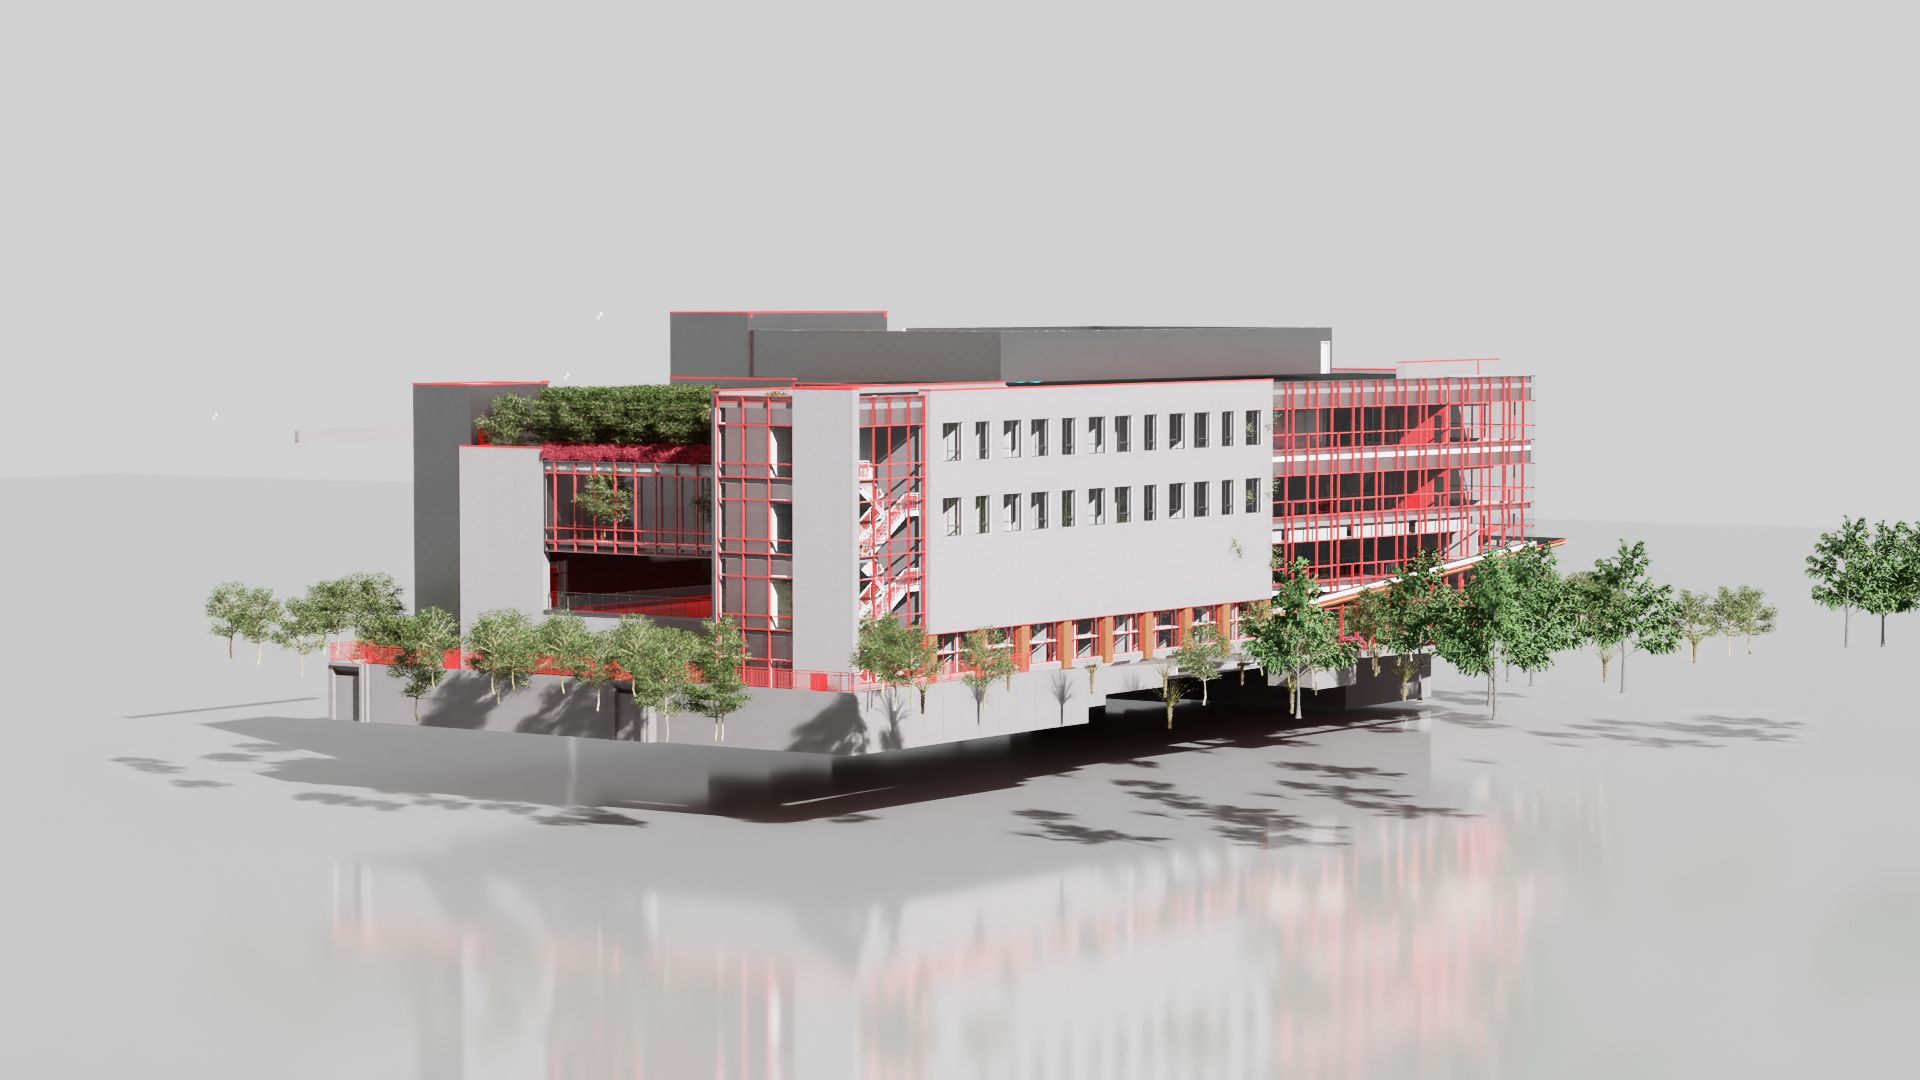
\includegraphics[width=\linewidth]{figures/innovation_center_exterior.png}
  \caption{The Robert D. Kern Engineering Innovation Center as a physics-accurate
  digital twin in NVIDIA Isaac Sim, rendered from the BIM-derived USD. The
  red-mullioned curtain wall, brick massing, landscaping, and per-floor interior
  structure are carried over directly from the Revit model --- the same geometry
  the robot navigates and the onboard camera perceives.}
  \label{fig:twin}
\end{figure}

\subsection{Scene Preparation}

\subsubsection{BIM-to-USD Conversion}

A major challenge was converting the Revit 2024 model to USD while preserving the
detail needed for downstream training. To optimize simulation performance, the
Revit model filtered non-essential systems (HVAC, electrical, plumbing),
retaining only structural components such as walls, floors, and doors. This
reduced file size from 818~MB to $\approx35$~MB and cut the number of elements
Isaac Sim must render. We exported with the NVIDIA Omniverse Connector with the
\emph{``Family Data Instancing''} setting enabled --- critical for preserving
individual building components as discrete objects (rather than a single fused
mesh), which maintains the semantic properties and structural hierarchy needed
for high-fidelity training and automatic per-element physics classification.

\subsubsection{Isaac Sim Scene and Physics}

The building USD is imported into Isaac Sim and organized as a reusable world
reference, so the architectural model functions as a simulation-ready
environment. Physics is then applied on top of NVIDIA PhysX, providing gravity,
rigid-body simulation, collision handling, and joint-based motion. Static
elements (walls, floors, glazing, stairs) are assigned \textbf{triangle-mesh
colliders} so the environment acts as a navigable physical space, while doors are
configured as \textbf{articulated rigid bodies with revolute joints and drive
controllers} for realistic opening behavior. Materials are grouped by surface
type so major components receive appropriate physical properties, and lighting
and rendering are configured through Isaac Sim's standard world-initialization
workflow.

Doors required particular care. An initial approach that guessed the hinge
location produced doors that clipped into walls. The working solution places the
hinge at the vertical edge of the door with a slight offset to avoid colliding
with the door's bounding box, and applies a drive motor with a per-class torque
limit (single- vs.\ double-leaf) tuned so the leaf opens cleanly on command. The full physics process --- element categorization, collider and
material assignment, and door articulation --- is implemented as a
\textbf{replicable, automated pipeline} that runs on any Revit-exported USD, which
is what makes the six-building digital campus feasible (\cref{sec:eval}).

\subsection{Occupancy Map, Navigation Graph, and Route Planning}
\label{sec:nav-graph}

Patrol navigation is built in three stages: an occupancy map is generated by
ray-tracing the twin, a navigation graph is placed on it with NVIDIA SWAGGER, and
patrol routes are computed over the graph.

\noindent\textbf{Occupancy mapping.}
For each floor, the USD scene is loaded into Isaac Sim and the
\texttt{isaacsim.asset.gen.omap} extension performs a raycast-based scan from a
grid of origin points. Each cell is labeled free, occupied, or unknown. Door
primitives are excluded from the collision layer during scanning so rays can pass
through doorways and reach inside rooms. The scanner runs multiple passes, seeding
additional origin points inside remaining unknown regions and stopping
automatically once the unknown fraction drops below $\sim0.5\%$ of the floor grid
or stops improving between passes (a handful of cells behind walls remain
permanently unreachable). Across the Innovation Center this uses
\textbf{75--175 scan origins per floor} (125 on floor~4) over a
$102.6\,\text{m}\times100.3\,\text{m}$ footprint, leaving under $2\%$ of each
floor grid unknown ($0.86\%$ on floor~4) for $\mathbf{{\sim}99\%}$ mean floor
coverage. Maps are
produced at $0.05$~m/pixel and exported as a grayscale PNG (black = wall, white =
free, grey = unknown), a NumPy array, and a metadata file. The PNG is written in
the ROS \texttt{map\_server} convention (row~0 = world $y_{\max}$; origin is the
world pose of the bottom-left pixel) so it can be consumed directly by Nav2
without remapping.

\noindent\textbf{Navigation graph (NVIDIA SWAGGER).}
The binary occupancy map is passed to NVIDIA SWAGGER, which places navigation
nodes through a multi-stage pipeline: (i) \emph{skeletonization} (a medial-axis
transform) reduces corridors to one-pixel-wide center lines; (ii) \emph{skeleton
sampling} places nodes at fixed endpoints and junctions plus regular intervals
along branches; (iii) \emph{free-space sampling} adds nodes inside large open
areas such as atriums and lecture halls; (iv) \emph{triangulation} introduces more
direct edges between mutually visible nodes; and (v) \emph{pruning} removes
redundant nodes/edges and discards disconnected subgraphs shorter than a minimum
length. Because skeletonization is sensitive to visual noise, a clean binary
occupancy map (not a raw architectural drawing with text, door arcs, and dashed
lines) is required to avoid tangled graphs. The resulting per-floor graphs range
from 219~nodes / 226~edges (floor~4) to 586~nodes / 589~edges (floor~3). Node
positions are stored in world coordinates with edges pre-weighted by Euclidean
distance, so the graph is usable in simulation without further coordinate
conversion.

\noindent\textbf{Door labeling and route planning.}
Using each door's position, the nearest graph node is labeled a \emph{door node}
(e.g., 57 doors collapsing to 47 unique door nodes on floor~4). A patrol that
inspects every door is then a
traveling-salesman problem (TSP) over the door nodes. We first run
\textbf{Dijkstra's algorithm}~\cite{dijkstra1959note} from each node to build a
complete all-pairs distance table that reflects true travel distance through
corridors. We generate an initial tour with a \textbf{greedy nearest-neighbor}
heuristic, improve it with \textbf{2-opt} local search (which uncrosses
self-intersecting routes by removing two edges and reconnecting), and repeat from
multiple starting nodes (\textbf{random restart}, 10 trials), keeping the best
tour. TSP is NP-hard, so this yields an efficient --- not provably optimal ---
route. Finally, each door-to-door leg of the chosen tour is expanded into a full
corridor path via Dijkstra shortest path, and the entire expanded waypoint
sequence is handed to the navigation stack as a single goal
(\cref{sec:nav2}).

\begin{figure*}[t]
  \centering
  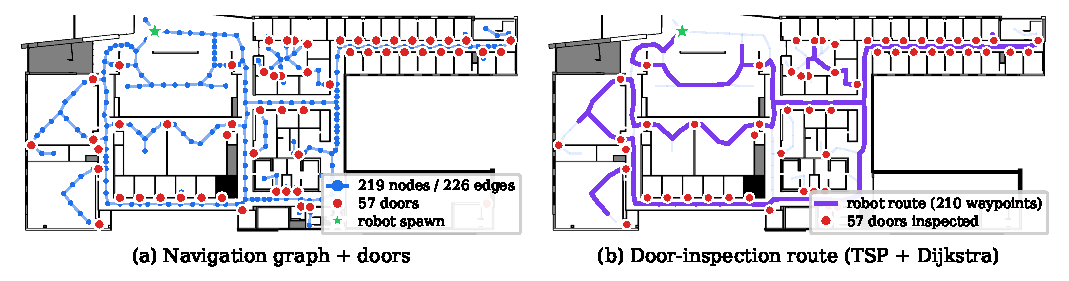
\includegraphics[width=0.92\linewidth]{figures/fig_navgraph.pdf}
  \caption{Occupancy map, navigation graph, and optimized door-inspection route
  on Innovation Center floor~4. (a)~the SWAGGER navigation graph (219 nodes /
  226 edges) with the 57 doors marked at their true world positions (each door is
  assigned the nearest graph node, giving 47 unique door nodes for the tour);
  (b)~the door-inspection tour (greedy nearest-neighbor + 2-opt) expanded by
  Dijkstra shortest paths into the 210-waypoint route the robot actually drives
  through the corridors.}
  \label{fig:navgraph}
\end{figure*}

\subsection{Local Navigation with ROS\,2 Nav2}
\label{sec:nav2}

Between waypoints, the robot drives itself with the \textbf{ROS\,2 Nav2} stack
(ROS\,2 Jazzy). Isaac Sim and Nav2 communicate through Isaac Sim's built-in
ROS\,2 bridge: the simulator publishes sensor streams and odometry, Nav2 publishes
velocity commands, and the simulated Nova Carter executes them. The TSP-expanded
route is sent as one \texttt{NavigateThroughPoses} action goal, so the robot
drives the full patrol continuously rather than stopping at each waypoint.

\noindent\textbf{Robot platform.}
The NVIDIA Nova Carter is a differential-drive mobile robot
($0.722\,\text{m}\times0.500\,\text{m}\times0.556\,\text{m}$, $51.2$~kg) on the
Segway RMP Lite 220 chassis (wheel radius $0.14$~m, wheel base $0.4$~m). Its
sensor suite includes a Hesai 3D LiDAR, front and rear 2D scanning LiDARs, four
stereo cameras, and an IMU, with onboard compute from an NVIDIA Jetson AGX Orin.
We use it because it has a validated USD model in the NVIDIA asset library and a
native ROS\,2 driver, so the same platform and command interface are used in
simulation and (planned) physical deployment, minimizing the sim-to-real gap for
locomotion. For perception we additionally mount a forward-facing first-person RGB
camera ($640\times480$, $15$~fps, $5$~mm focal length) that always points in the
direction of travel; this is the input to the VLM (\cref{sec:vlm}).

\noindent\textbf{Sensing and localization.}
The Hesai 3D LiDAR point cloud is projected to a 2D \texttt{LaserScan}
(\texttt{/scan}) via \texttt{pointcloud\_to\_laserscan} and feeds the global
obstacle costmap; the front/rear 2D LiDARs feed the local costmap. Localization
uses \textbf{AMCL} (Adaptive Monte Carlo Localization) against the static map
produced in \cref{sec:nav-graph}, with a differential motion model. The global
planner is \textbf{SmacPlanner2D} (A* with cost-weighted edge selection) and the
local controller is the \textbf{Dynamic Window Approach} (DWB); recovery and
replanning are handled by the standard Nav2 behavior tree. Costmaps are layered: a
global static + obstacle + inflation costmap over the whole floor, and a rolling
$6\,\text{m}\times6\,\text{m}$ local costmap fusing the 2D scans, a 3D voxel
layer, and inflation.

\noindent\textbf{Parameter choices that matter.}
Off-the-shelf Nav2 parameters did not work in long architectural corridors; the
changes in \cref{tab:nav2} were needed and are reported so others can reproduce
them. Maximum commanded velocity is $1.6$~m/s linear and $1.1$~rad/s angular.
Goal tolerance is $0.25$~m / $0.25$~rad with a stateful goal checker so a
multi-pose tour tolerates small drift.

\begin{table}[t]
  \centering
  \small
  \begin{tabular}{@{}p{2.55cm}rrp{2.0cm}@{}}
    \toprule
    \textbf{Parameter} & \textbf{Upstream} & \textbf{Ours} & \textbf{Effect} \\
    \midrule
    \texttt{collision\_} \texttt{monitor} \texttt{min\_points} & $6\!\times\!10^{9}$ & \textbf{4} & Re-enables the emergency stop \\[2pt]
    DWB \texttt{Base} \texttt{Obstacle.scale} & 0.02 & \textbf{15.0} & Robot swerves around obstacles \\[2pt]
    obstacle / raytrace range & 10.0\,m & \textbf{15.0\,m} & Plans global detours early \\[2pt]
    \texttt{cost\_travel\_} \texttt{multiplier} & 2.0 & \textbf{4.0} & Prefers wall-clearing cells \\
    \bottomrule
  \end{tabular}
  \caption{Deliberate Nav2 parameter changes relative to the upstream Nova Carter
  defaults, with their effect in long architectural corridors.}
  \label{tab:nav2}
\end{table}

\begin{figure}[t]
  \centering
  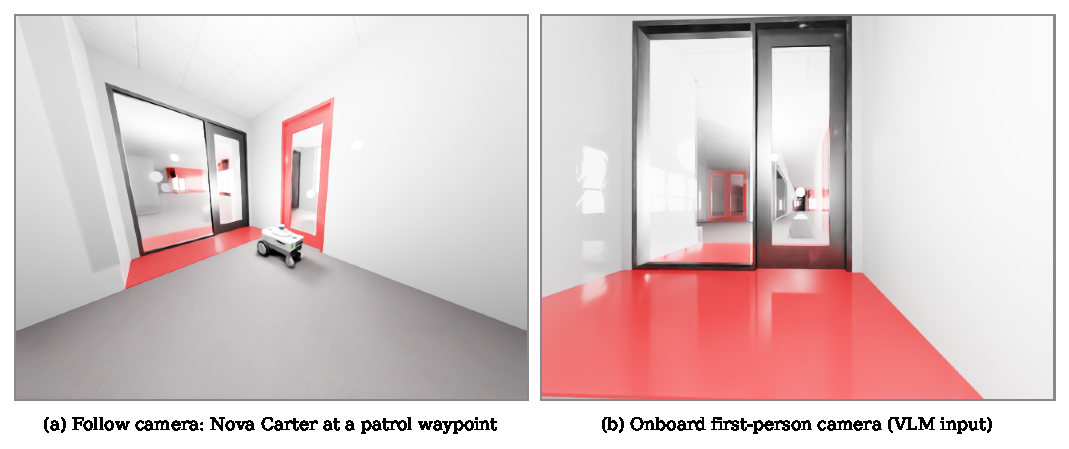
\includegraphics[width=\linewidth]{figures/fig_nav2.pdf}
  \caption{The deployed stack in action: real frames from a floor-4 patrol run
  in which ROS\,2 Nav2 autonomously drives the Nova Carter robot between
  inspection waypoints in the BIM-derived twin. (a) Third-person follow camera
  with the robot stopped at a glass-door waypoint; (b) its forward-facing
  first-person camera---the input to the VLM (\cref{sec:vlm})---viewing the
  closed glass door it has reached. Both are rendered sensor streams from the
  same run, not illustrations.}
  \label{fig:nav2}
\end{figure}

\subsection{Vision-Language Perception}
\label{sec:vlm}

To give the robot semantic awareness, we fine-tune a vision-language model to
classify anomalies in the onboard camera stream. We reached out to MSOE Public
Safety for the anomalies they look for during walkthroughs and targeted the
\textbf{top two}: doors left \textbf{open/unsecured} and \textbf{cracked glass}.
The model is asked a single four-way question --- \emph{door open, door closed,
glass cracked, or glass intact} --- so one model covers both anomaly types while
still describing the rest of the scene for free.

\noindent\textbf{Why a VLM.}
Unlike a CNN classifier, a VLM already knows what a hallway, student, or fire
extinguisher is, so fine-tuning only the anomaly behavior leaves its general world
knowledge intact, and it can explain a flag in natural language to a human
operator rather than emit a bare probability.

\noindent\textbf{Synthetic data from the twin.}
Because the building is not yet built, we cannot photograph it; and even for built
spaces one cannot stage break-ins, floods, or fires on demand. Instead we
manipulate the twin's internal state to \emph{program} each anomaly and read the
ground-truth label directly from the simulator --- a free, exact label for every
frame. Doors are articulated revolute joints, so the ground-truth door angle is
queried from the joint and thresholded ($\le5^\circ$ closed, $>5^\circ$ open).
Cracked glass is rendered by swapping the material on a random subset of glass
panels to a cracked variant each frame; Replicator emits the corresponding
semantic-segmentation labels.

The \textbf{cracked-glass pipeline} is visual-only (no geometry fracture). Of the
$\sim1{,}013$ glass panels in the Innovation Center USD, the standard double-pane,
curtain-wall, and glazed system panels are crackable (shadowbox and laminated
panels are excluded). Each cracked panel is rendered with an OmniGlass shader
whose \texttt{normal\_map\_texture} input is wired to a crack normal map, swapped
per frame through direct material binding so the binding and the semantic label
stay consistent. Three crack styles provide variety: a physics-grounded
\emph{tempered} style (Voronoi tessellation matching real tempered-glass
fracture), an \emph{impact} style (spider-web cracks generated by Stable Diffusion
XL line-art passed through a Sobel filter into a normal map), and an \emph{edge}
style (a branching random walk from a panel edge), all illustrated on the same
panel in \cref{fig:synthdata}. Domain randomization spans lighting presets, the
fraction of panels cracked per frame, the tiling/impact-point toggle, and camera
pose.

\begin{figure*}[t]
  \centering
  % TODO(figure): swap these tight crops of the panel00 renders for the
  % real high-res heavy-shatter frames from datasets/cracked_glass/<run>/rgb/
  % (on another machine; not in this checkout). Regenerate via
  % docs/paper/figures_src/make_synthdata.py.
  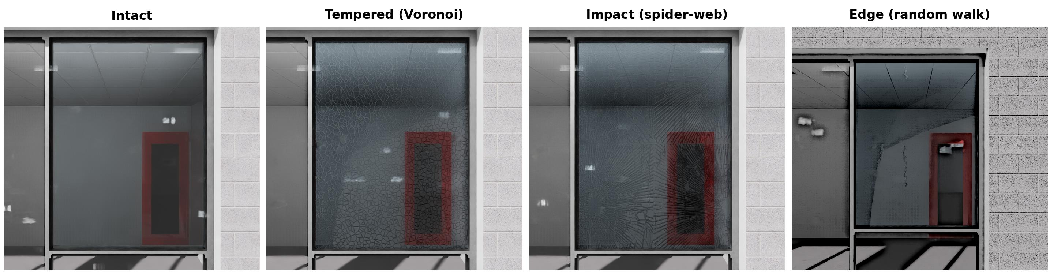
\includegraphics[width=0.92\linewidth]{figures/fig_synthdata.pdf}
  \caption{Synthetic anomaly data rendered from the digital twin's onboard
  robot camera. The same curtain-wall panel is shown intact and with the three
  crack styles (tempered Voronoi, impact spider-web, edge random-walk). Because
  the anomaly is programmed into the twin, every frame carries an exact,
  free ground-truth label.}
  \label{fig:synthdata}
\end{figure*}

The \textbf{door pipeline} holds a door at a fixed angle per episode and captures
frames from a multi-camera arc; per-episode angle randomization produces a smooth
spread of openness. Critically, the dataset spans \textbf{multiple doors and door
families} --- 8 training doors across Revit families (CW\_F, CW\_FG, Type\_F,
Type\_N, Type\_FG), plus 2 held-out doors (an unseen instance and an unseen swing
direction) --- under six lighting presets and varied viewpoint/height. This
multi-door, randomized design is a direct response to a generalization failure in
an earlier single-door dataset (\cref{sec:vlm-eval}).

\noindent\textbf{Model and fine-tuning.}
The backbone is \textbf{Qwen3-VL-2B-Instruct}. We apply \textbf{LoRA} (rank 16,
$\alpha$~32, dropout 0.05) to the language backbone's \texttt{q\_proj} and
\texttt{v\_proj}, and additionally \textbf{co-train the full vision projector}
(the \texttt{visual.merger} patch-merger) via PEFT's \texttt{modules\_to\_save}.
The projector is the bridge between visual patch tokens and the LLM's embedding
space; the base projector was optimized for real photographs, and without adapting
it the LLM receives no meaningful information about synthetic door/glass state ---
no amount of LoRA training compensates. In total $\approx\mathbf{1.62\%}$ of
parameters are trained ($\approx2.2$M LoRA + $\approx34$M projector). Training runs
on a Tesla V100 (Rosie \texttt{dgx} partition). Two engineering pitfalls were
essential to get right: PEFT's default save drops the trained projector weights
unless they are listed in \texttt{modules\_to\_save} (the symptom is a model that
silently reverts to the untrained baseline), and trainable projector parameters
must be cast to fp32 for AMP gradient scaling.

\section{Evaluation}
\label{sec:eval}

\subsection{Scene Fidelity}

The converted USD scene preserves the source Revit model's structural elements,
semantic metadata, and spatial organization, which lets the automated physics
pipeline classify elements by parent folder rather than by manual annotation.
Functional accuracy is verified through three automated strategies. \emph{Drop
testing} discovers floor levels by clustering floor-element bounding boxes by
$Z$-coordinate, spawns rigid bodies above each surface, and samples their $Z$ over
time to distinguish objects that come to rest (solid collider) from objects that
fall through (missing collider). \emph{Robot-in-the-loop validation} drives a robot
in a patrol pattern on each surface while monitoring its $Z$, exposing surface
gaps during active motion. \emph{Automated visual validation} records an orbital
$360^\circ$ sweep for manual inspection of overall form and physics behavior
across levels.

\subsection{Navigation Graph Coverage}

Occupancy maps were produced for all four above-ground floors. Unknown cells
ranged from $0.47\%$ (floor~1) to $1.65\%$ (floor~2) --- under $2\%$ on every
floor --- for ${\sim}99\%$ mean floor coverage at $0.05$~m/pixel ($0.86\%$
unknown on floor~4). We validated floor~4 by overlaying the computed
world coordinates onto the occupancy image and confirming in NVIDIA Omniverse that
every navigation node falls in free space, not inside walls or obstacles. Route
correctness was demonstrated with Dijkstra's shortest path traversing the full
layout, and full-floor reachability was confirmed by the TSP solution (greedy
nearest-neighbor + 2-opt + random restart) visiting every door node.

\subsection{Navigation and Route Execution}

Driving the SWAGGER route with Nav2 inside the twin, the Nova Carter follows the
planned door-inspection tour and avoids obstacles in real time using its LiDAR
costmaps. We exercise the stack at three route scales --- single-wing (easy),
cross-wing (medium), and full-building (hard) --- and with adversarial obstacles
spawned in corridors at known world coordinates. With the tuned parameters of
\cref{sec:nav2} the robot completes routes and recovers from blocked corridors via
the Nav2 behavior tree; with the upstream defaults it either disables its
emergency stop or drives through obstacles, motivating the changes we report.

A full quantitative characterization --- per-scale route completion rate, mean
path length relative to the graph-optimal tour, number of recovery behaviors
triggered, and obstacle-avoidance success rate --- is the focus of an ongoing
evaluation campaign and is the primary remaining gap before physical deployment.

\subsection{Vision-Language Perception Evaluation}
\label{sec:vlm-eval}

\begin{figure*}[t]
  \centering
  % TODO(figure): door/glass held-out cell counts are reconstructed under a
  % balanced-class assumption (the eval IS stratified 50/50, so this is exact in
  % method, +/-1 from rounded per-class %). Replace with exact integers from
  % data/finetuned_eval_results.json (on another machine) when available.
  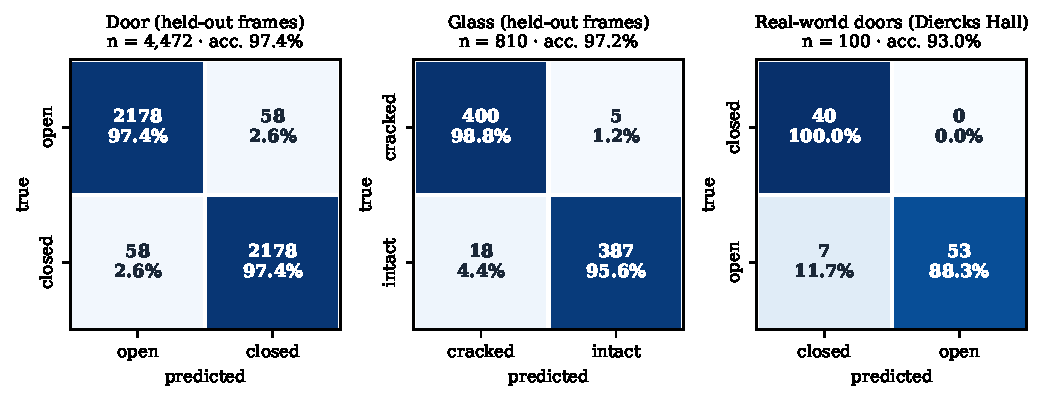
\includegraphics[width=0.82\linewidth]{figures/fig_confusion.pdf}
  \caption{Confusion matrices for the fine-tuned Qwen3-VL-2B model on the
  held-out door, held-out glass, and real-world Diercks Hall door test sets
  (rows: true class; cells: count and per-class recall). The real-world split is
  exact; counts for the two synthetic splits are reconstructed from the reported
  per-class accuracies under a balanced-class assumption, which reproduces the
  overall accuracies of \cref{tab:vlm}.}
  \label{fig:vlm}
\end{figure*}

\noindent\textbf{Model selection (zero-shot baselines).}
We first evaluated several small open VLMs zero-shot on synthetic door frames. No
off-the-shelf model is usable as-is, and Qwen3-VL-2B is both the strongest and the
smallest deployable option (\cref{tab:baselines}).

\begin{table}[t]
  \centering
  \small
  \begin{tabular}{@{}lcc@{}}
    \toprule
    \textbf{Model} & \textbf{Params} & \textbf{Zero-shot acc.} \\
    \midrule
    Qwen3-VL-2B-Instruct        & 2B   & \textbf{69.3\%} \\
    Qwen2.5-VL-7B-Instruct$^{*}$ & 7B   & 68.7\% \\
    Qwen2.5-VL-3B-Instruct      & 3B   & 64.9\% \\
    InternVL3-2B                & 2B   & 62.9\% \\
    Qwen2-VL-2B-Instruct        & 2B   & 62.1\% \\
    SmolVLM2-2.2B-Instruct$^{*}$ & 2.2B & 62.1\% \\
    \bottomrule
  \end{tabular}
  \caption{Zero-shot door-state accuracy of small open VLMs.
  $^{*}$evaluated on the brighter-lighting subset.}
  \label{tab:baselines}
\end{table}

\noindent\textbf{Fine-tuned accuracy.}
After LoRA + projector co-training, the unified Qwen3-VL-2B model reaches
$\mathbf{97.4\%}$ on held-out door frames ($n=4{,}472$; open $97.4\%$, closed
$97.4\%$) and $\mathbf{97.2\%}$ on held-out glass frames ($n=810$; cracked
$98.8\%$, intact $95.6\%$). The glass gain is the clearest evidence that
fine-tuning, not the base model, does the work: zero-shot glass accuracy is only
$37.6\%$ (near chance), which co-training lifts to $97.2\%$. \Cref{tab:vlm}
summarizes performance across test sets, including the out-of-distribution and
real-world transfer tests.

\begin{table}[t]
  \centering
  \small
  \begin{tabular}{@{}lrcc@{}}
    \toprule
    \textbf{Test set} & $\mathbf{n}$ & \textbf{Zero-shot} & \textbf{Fine-tuned} \\
    \midrule
    Door (held-out frames)         & 4{,}472 & ---     & \textbf{97.4\%} \\
    Glass (held-out frames)        &   810   & 37.6\%  & \textbf{97.2\%} \\
    Door (held-out inst./swing)    & 7{,}776 & 84.1\%  & \textbf{90.2\%} \\
    Real-world doors (Diercks Hall)&   100   & ---     & \textbf{93.0\%} \\
    Real-world glass (Diercks Hall)$^{\dagger}$ & 100 & --- & \textbf{81.0\%} \\
    \bottomrule
  \end{tabular}
  \caption{Fine-tuned Qwen3-VL-2B accuracy across held-out, out-of-distribution,
  and real-world test sets. $^{\dagger}$The real-world glass set comprises
  photographs of intact glass in Diercks Hall with crack patterns applied by a
  diffusion model (Gemini), not photographs of physically cracked glass.}
  \label{tab:vlm}
\end{table}

\noindent\textbf{Generalization is the central result.}
An earlier single-door, single-family dataset reached high in-distribution
accuracy but collapsed to $\mathbf{0\%}$ on a door instance it had never seen ---
it had memorized one door's appearance, not the concept of open vs.\ closed. This
failure motivated the multi-door, multi-family, domain-randomized dataset
described in \cref{sec:vlm}. The current model retains $\mathbf{90.2\%}$ on a
held-out test that mixes an unseen door instance and an unseen swing direction (up
from $84.1\%$ zero-shot), demonstrating that diverse synthetic training, not
memorization, drives the result.

\noindent\textbf{Real-world transfer.}
We tested on \textbf{100 real photographs of doors in Diercks Hall}, an existing
MSOE building designed by the same architect with the same general design language
as the Innovation Center. Trained only on synthetic imagery, the model reaches
$\mathbf{93.0\%}$ (closed $100\%$, open $88.3\%$), confirming that the
digital-twin-only training pipeline transfers to real buildings. We additionally
evaluated glass on $100$ Diercks Hall images in which a diffusion model (Gemini)
applied crack patterns to photographs of intact glass --- a semi-synthetic test,
since physically cracked glass cannot be staged on demand. Here the model reaches
$\mathbf{81.0\%}$ (intact $100\%$, cracked $62.0\%$): real-glass intact frames
transfer perfectly, but the diffusion-applied cracks differ enough from the twin's
procedural cracks that cracked-glass recall drops, indicating the glass branch is
more sensitive to the crack-appearance domain gap than the door branch.

\section{Discussion}

\subsection{Limitations}
The simulation models static building geometry without dynamic occupants
(students, staff, transient furniture) that would be present during real patrol.
Patrol routes are currently planar (per-floor); vertical transitions via elevators
and stairwells are not yet integrated into the graph. The BIM-to-USD conversion
still requires some manual intervention for certain Revit export conditions, which
bounds how quickly a new building can be onboarded. Quantitative Nav2
route-execution metrics are still being tabulated. Finally, the strongest
perception result is on doors; cracked-glass detection is validated on synthetic
held-out frames ($97.2\%$) and on diffusion-edited real-glass imagery ($81.0\%$,
with cracked recall falling to $62.0\%$), but not yet on photographs of physically
cracked glass --- closing that crack-appearance domain gap is future work.

\subsection{Sim-to-Real Transfer}
Using the same Nova Carter platform and ROS\,2 command interface in simulation and
deployment minimizes locomotion-dynamics mismatch, but several domain-shift
sources remain: floor-surface texture/friction and minor elevation changes,
sensor-noise characteristics of the physical LiDARs (not replicated in the
raycaster), real-facility lighting, and --- most significantly --- dynamic
occupants absent from the training distribution. On the perception side, the
$93.0\%$ real-world door result is strong evidence the synthetic pipeline
transfers. For real deployment, robust on-boot localization is needed because the
robot is initially blind to its pose; Nova Carter's LiDAR, wheel encoders, and
cameras support a SLAM solution to construct and localize within a map,
complementing the prior-map AMCL used in simulation.

\subsection{Future Work}
The most immediate extensions are quantitative Nav2 patrol evaluation in the full
building, real-world cracked-glass validation, and extending the navigation graph
across floors with elevators and stairwells for full-building coverage. The Kern
Center recreation facility will serve as a second evaluation building and the
first cross-building generalization test. Physical deployment trials on Nova
Carter, supervised by the Public Safety Office, will provide the first real-world
validation of the end-to-end pipeline. More broadly, the six-building digital
campus is a reusable substrate for tasks well beyond patrol.

\section{Conclusion}

We presented a framework for automatically deriving robot training environments
from Building Information Modeling data, eliminating manual scene authoring.
Starting from a Revit BIM file, the pipeline converts geometry to USD, loads it
into NVIDIA Isaac Sim as a physics-accurate digital twin, extracts an occupancy
map and a SWAGGER navigation graph for traveling-salesman patrol planning, drives
a Nova Carter robot along those routes with ROS\,2 Nav2, and fine-tunes a
Qwen3-VL-2B model on synthetic imagery to detect open doors and cracked glass ---
transferring to real-world building imagery at $93.0\%$ accuracy. The physics
pipeline is fully automated: it takes an architecture file as input and produces a
physics-ready digital twin, which let us build a \textbf{six-building digital
campus} consuming over \textbf{3{,}500 GPU jobs and 2{,}000 GPU-hours} on MSOE's
Rosie supercomputer. Any facility whose BIM model exists becomes a candidate for
site-specific robot training before its doors ever open.

{
    \small
    \bibliographystyle{ieeenat_fullname}
    \bibliography{paper}
}

\end{document}
